\mysubsection{Sources de données}

\ifbook{
  \mysubsubsection{Qu'est ce qu'une ressource ?}

\paragraph{} Dans le domaine du \textit{middleware}, on utilise régulièrement des abstractions, du
plus au niveaux possibles, pour créer des composants les plus génériques possibles, pouvant donc
être ainsi réutilisé autant que possible. En outre, ces composants peuvent être configurés pour
répondre à des problématiques similaires. Une de ces abstractions les plus courament utilisée est la
notion de \textbf{ressource}\footnote{Là encore, l'expérience très orientée Java/JEE de l'auteur de
ce document influence peut être la sémantique. Fort heureusement, les concepts décrits ici devraient
pouvoir s'appliquer à toutes autres technologies.}.

\paragraph{} Une ressource désigne en fait une application tierse, un service au sens le
plus générique du terme, que l'application accède pour transmettre et recevoir des donnnées. Une
ressource peut donc être un simple fichier ou quelquechose d'aussi complexe qu'une base de données
relationnelle.

\paragraph{} Les entités désignées par ce terme sont volontairement très abstraite pour permettre d'
utiliser élements ou mécanismes de nature très différentes d'une manière identique. Mais, aussi
abstrait soient elles, les ressources partagent tout de même certains point en communs:

\begin{description}
  \item[processus externe] une \textbf{ressource} est forcément externe au
  processus de l'appication. Un cache local, par exemple, même s'exécutant dans un processus séparé,
  ne peut pas réellement être considéré comme \textbf{ressource}. Si le cache est dans une
  application séparée - par exemple une instance de \mylink{TODO}{MemCached} s'exécutant sur un
  autre serveur que l'application, il peut alors être considéré comme une \textbf{ressource}.
  \item[entrées/sorties] Par nature, une \textbf{ressource} est donc sources d'entrées/sorties. Un
  échange de données est effectué entre l'application et cette dernière. Ce postulat implique qu'il
  faut donc gérer, la plupart du temps, une forme de connexion (ou un \textit{pool} de connexion)
  vers cette dernière. Bien évidemment, comme évoqué déjà plus en amont du cours, avec un
  tel échange, la notion de \textbf{transaction} ne tarde pas à apparaitre, et, avant elle, les
  problématiques d'\textbf{authentification} et de \textbf{sécurité}...
\end{description}
}

\ifslide{
  \begin{frame}{Les ressources}
    \begin{block}{Qu'est ce qu'une ressource ?}
      \begin{itemize}
        \item une base de données (\textit{of course})
        \item un fichier
        \item la ressource désignée par une URL
        \item un fichier dans le classpath !
        \item ...
      \end{itemize}
    \end{block}
  \end{frame}

  \begin{frame}{Source de données}
    \begin{center}
      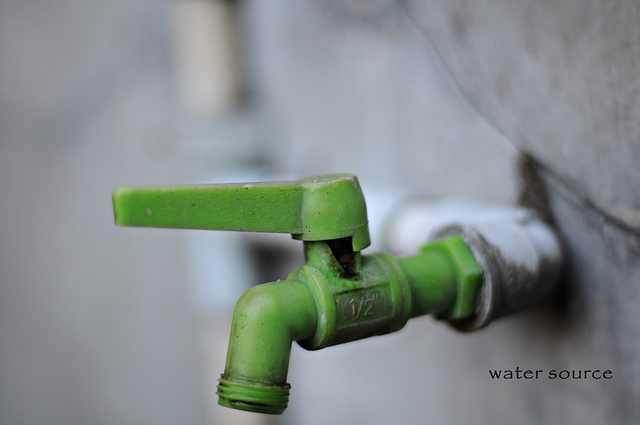
\includegraphics[scale=0.2]{../img/tapwater.jpg}
    \end{center}

    \begin{block}{Caractéristiques}
      \begin{itemize}
        \item externe au processus d'exécution du programme
        \begin{itemize}
          \item un cache local n'est pas, par exemple, une ressource
        \end{itemize}
        \item I/O
        \item doit être gérée:
        \begin{itemize}
          \item fermerture de connection (suivi des connections)
          \item transaction
          \item sécurité
        \end{itemize}
      \end{itemize}
    \end{block}
  \end{frame}
}

\ifbook{
  \mysubsubsection{Gestionnaire de connexion}

  \paragraph{} La notion de \textbf{ressource} étant définie - dans ses grandes lignes, nous allons
  maintenant évoquer brièvement un mécanisme qui leurs sont très souvent associé : les gestionnaires
  de connexion (souvent désigné par leur appelation anglaise de \textit{pool} de connexion).

  \paragraph{} Pour bien cerneur leur intérêt, il est nécessaire de comprendre que
  l'établissement d'une connexion à une resource - encore une fois qu'il s'agisse d'une base de
  données SQL ou d'un annuaire d'entreprise utilisant le protocole LDAP, est une opération
  \textbf{coûteuse}. En plus des coûts associés à la connexion réseau - les ressources étant souvent
  des application s'exécutant sur une machine séparée, toute la logique d'\textbf{authentification}
  et d'\textbf{indentification} qui leurs sont associées, ont généralement aussi un impact.

  \paragraph{} Fort de ce constat, il apparait pertinent de prémunir l'application utilisant une
  ressource d'être pénalisé en performance, en devant systématiquement ouvrir une nouvelle connexion
  à chaque requête. Et c'est à cette fin que la plupart des \textit{middlewares} proposent de
  disposer d'un \textit{pool} de connexion, prêt à l'emploi.

  \paragraph{} Ce dernier consiste en effet en ensemble de connexion pré établis. À chaque requête,
  l'application demande au gestionnaire de lui fournir une connexion par laquelle elle
  accèdera à la ressource. Une fois son travail effectué, elle restitue au gestionnaire la
  connexion, qui pourra donc la transmettre à un autre processus demandeur- qu'il s'agisse de la
  même application ou d'une autre.

  \paragraph{} Si la demande intervient à un moment où il n'y a aucune connexion de libre, la
  requête doit donc attendre qu'une connexion se libère pour finir de s'exécuter. De ce constat,
  deux points importants apparaisent immédiatement:

  \begin{enumerate}
    \item La présence d'un \textit{pool} de connexion protège la ressource vis à vis de ses
    consommateurs. Comme cette dernière est vraisemblablement partagée, ce mécanisme empêche une
    application connaissant une grave avarie ou un pic de charge inattendu, de soudainement rendre
    la ressource totalement inaccessible à ses autres utilisateurs.
    \item Par le même raisonnement, un \textit{pool} de connexion sous dimensionné formera
    rapidement le \textbf{goulot d'étranglement} de l'application, qui ne pourra répondre aux
    demandes de ses utilisateurs, puisqu'elle sera tout le temps en attente de libération de
    connexion.
  \end{enumerate}

  \paragraph{} C'est la raison pour laquelle les ressources, et spécialement les bases de données,
  forment souvent un goulot d'étranglement. On notera néanmoins qu'une application
  utilisant une ressource de manière abusive, en exécutant - par exemple, des requêtes SQL d'une
  complexité insensée, peut tout à fait être à la source du goulot d'étranglement, même si il
  apparait en extérieur que c'est la resource qui est à blâmer.\footnote{Encore une fois, si ce n'a
  pas déjà été fait, on soulignera que les problèmes de performances sont difficiles à cerner et à
  résoudre, et qu'il est important de ne pas juger de leur nature à "l'emporte pièce".}

}

\ifslide{
  \begin{frame}{Gestionnaire de connection}

    \begin{block}{\textit{Connection pooling}}
      \begin{itemize}
        \item ouverture de connection couteuse
        \item connections partagées
        \item prêtes à utiliser
      \end{itemize}
    \end{block}

    \begin{center}
      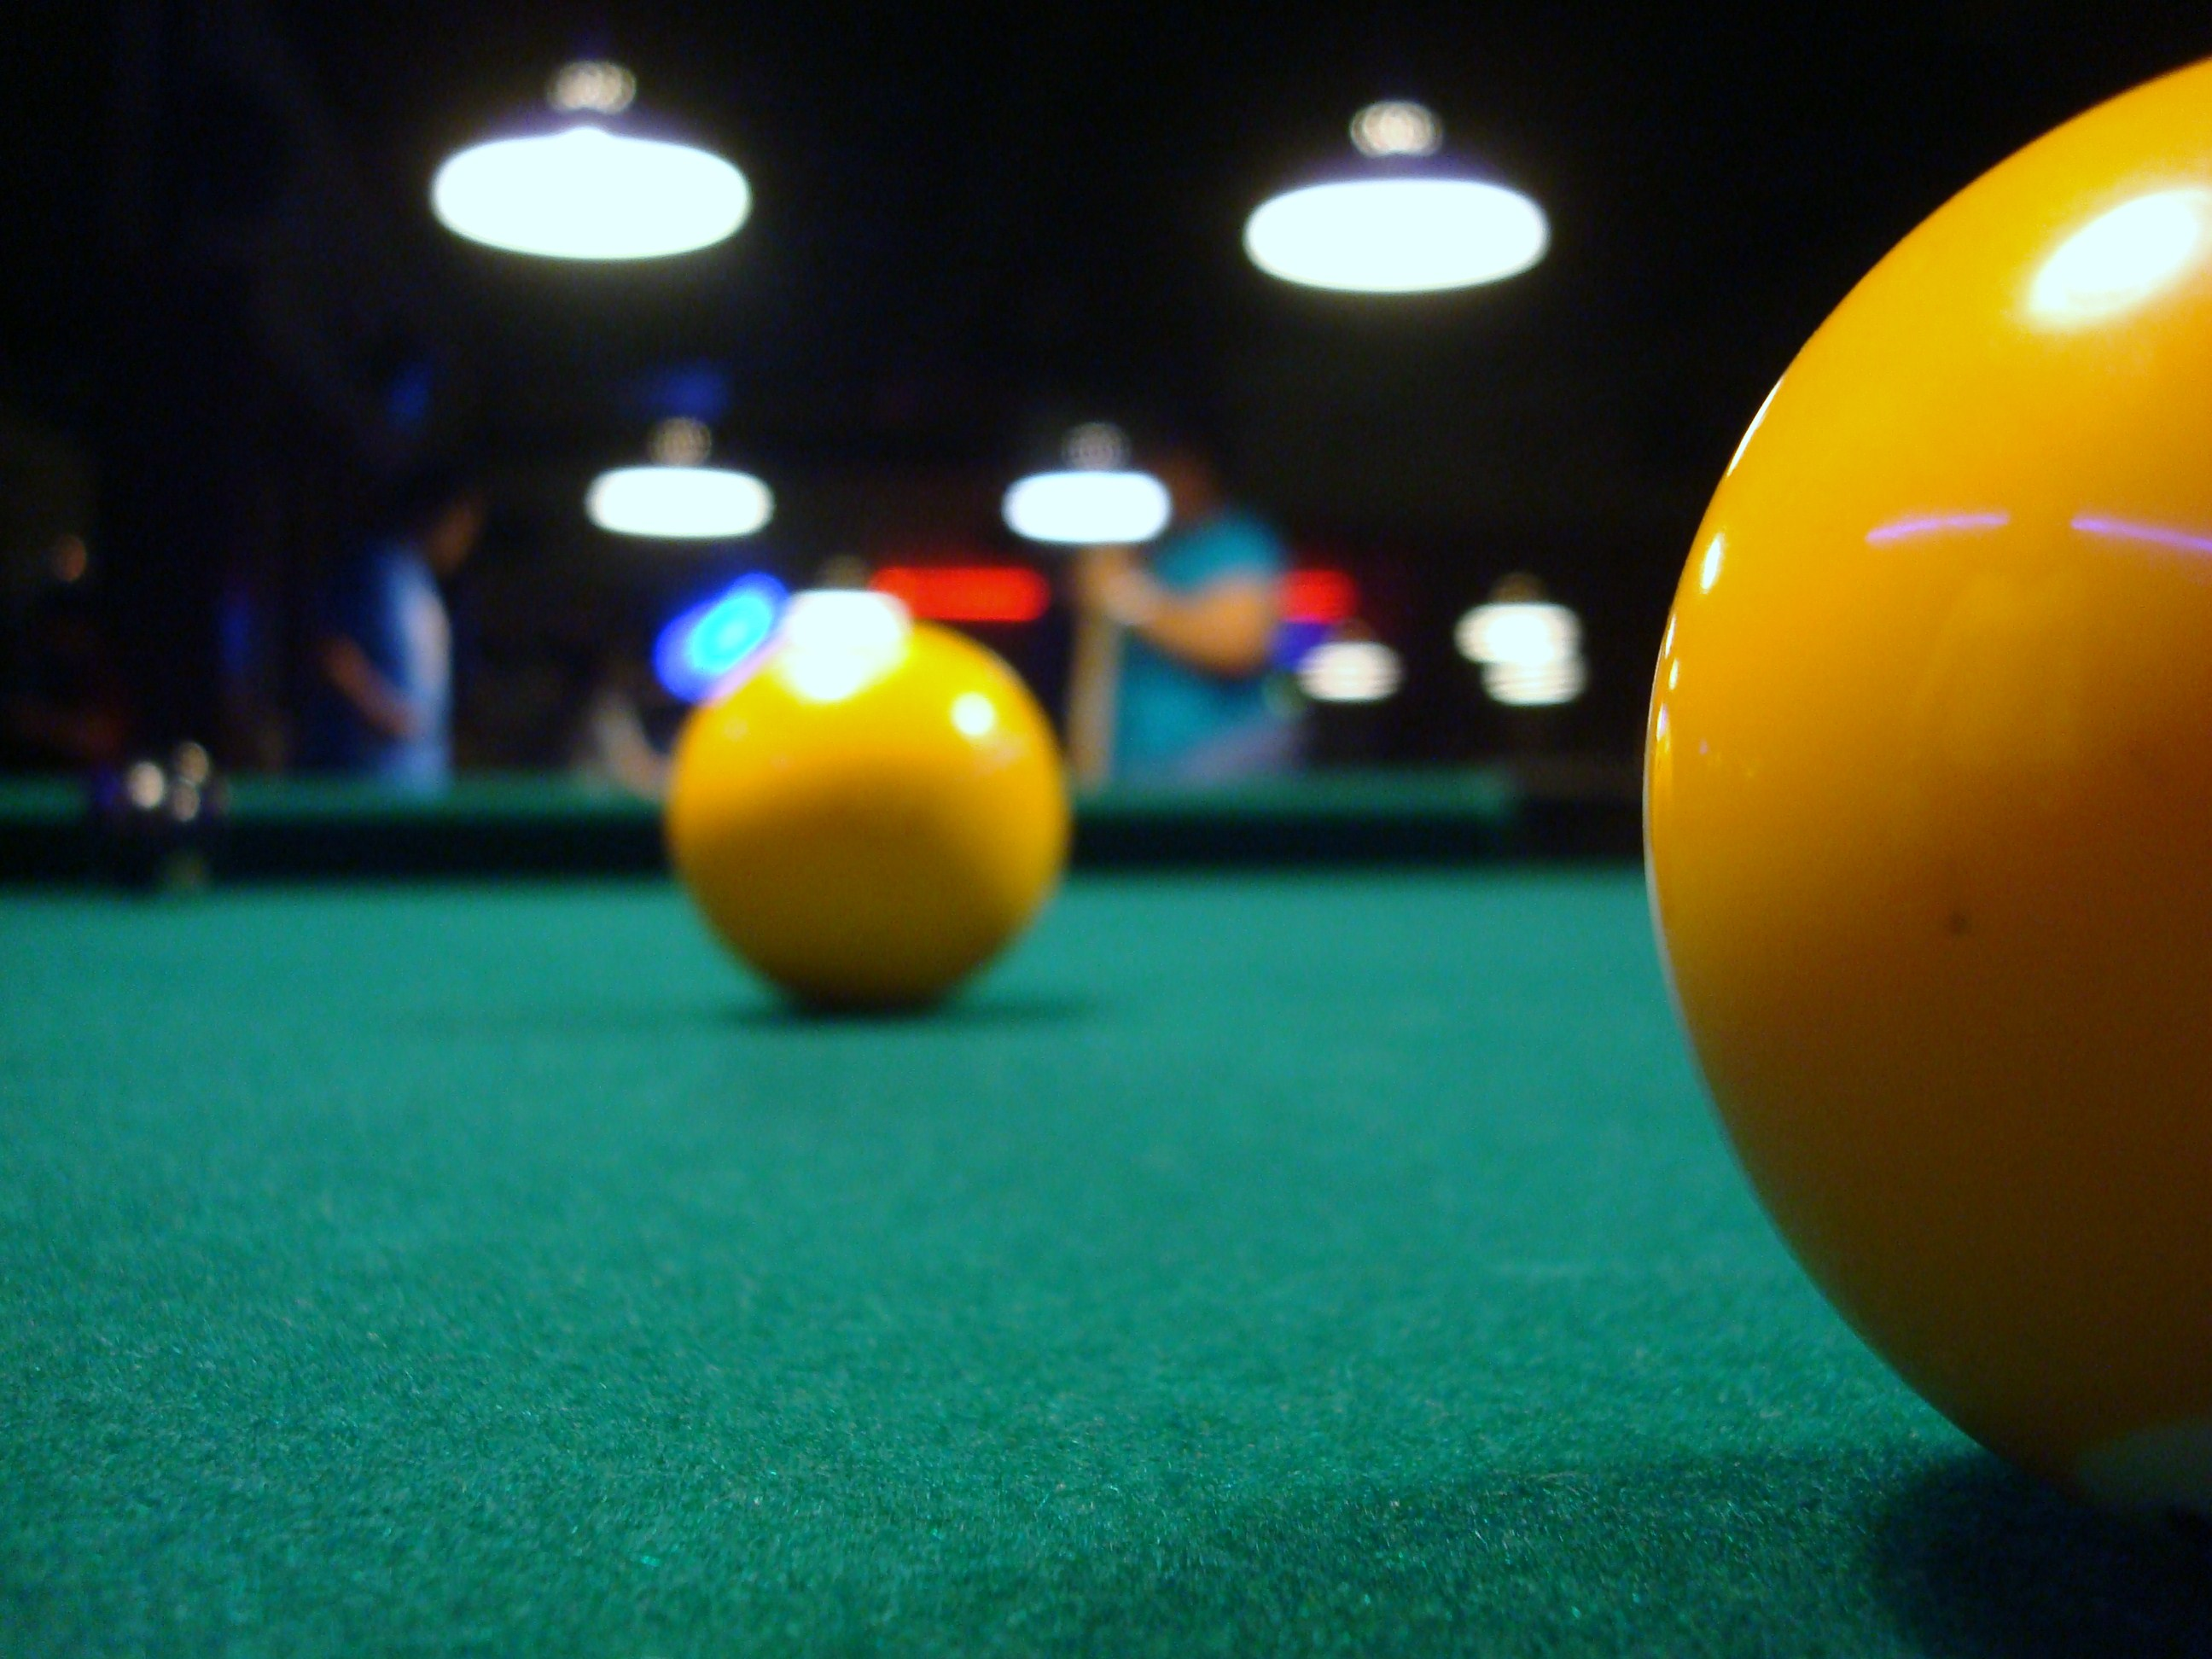
\includegraphics[scale=0.05]{../img/pool.jpg}
      \myphotocredit{http://www.flickr.com/photos/robertbanh/3294410460/sizes/o/in/photostream/}{Robert Banh}
    \end{center}

  \end{frame}
}


\ifbook{
  \paragraph{} Comme pour beacoup des thèmes abordés dans ce cours, des ouvrages entiers pourraient
  être écrit (et ont été écrits) sur le sujet de la gestion des ressources. Pour éclairer le lecteur
  de manière simple et pragmatique, nous allons donc remplacer ce potentiellement très long discours
  théorique, par l'étude de deux exemples concrets et pragmatiques d'utilisation de ressources.

  \paragraph{} Là encore, les exemples seront issues d'outils et de pratiques généralement associés
  à l'environement de développement et au cadre d'exécution Java, mais la logique sous jacente
  devrait se retrouver naturellement dans d'autres univers technologique, telle que C\# ou Python.

  \mysubsubsection{SQL et les base de données relationnelles}

  \paragraph{} Le premier exemple de ressource étudié est de loin le plus courament rencontré, car
  presque toutes les applications utilisent une base de données relationnelle pour persister ses
  données.

  \paragraph{} L'extrait de code Java ci dessous présente comment une application Java
  accède, de manière standard à une \textbf{source de  données}\footnote{Source de donnée est nom
  générique donnée aux bases de données}.

  \begin{center}
    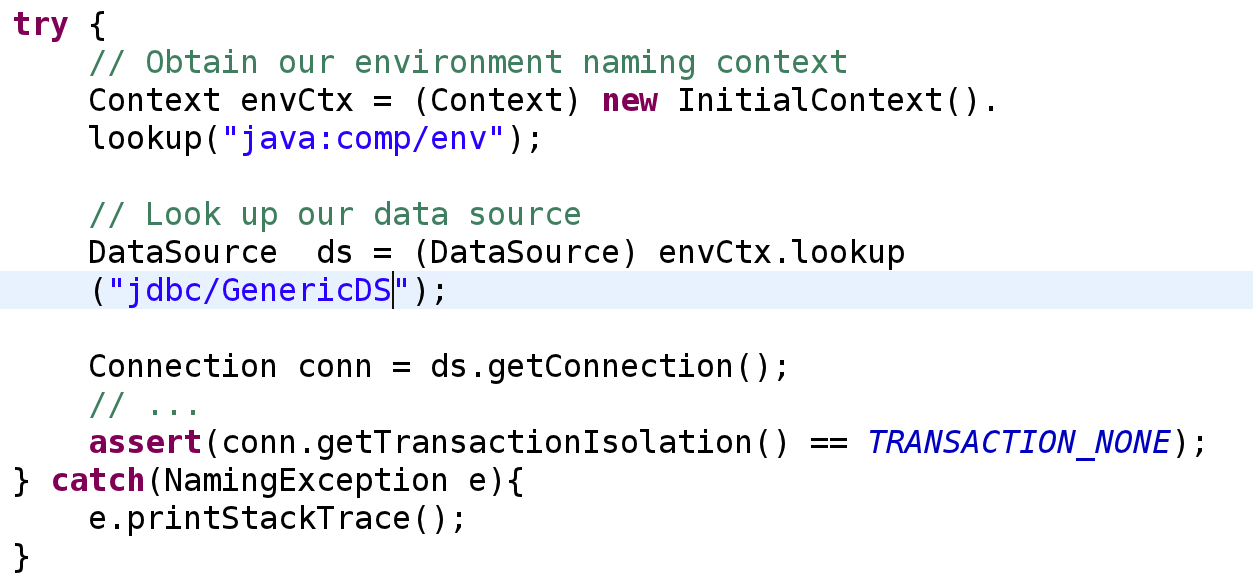
\includegraphics[scale=0.3]{img/datasource-connection.png}
  \end{center}

  \paragraph{} Il est important de remarquer que là encore, le souci d'abstraction apparait
  clairement. Le code présenté n'a en effet aucune dépendance à une API spécique à la base de
  données utilisée (Oracle, Postgresql,...). L'établissement de la connexion ne se fait que par
  l'utilisation d'un simple nom logique, désignant la ressource que l'on cherche à accéder. Le
  travail qui consiste à localiser cette ressource et à établir une connexion avec elle a été
  entièrement délégué au connecteur du conteneur d'exécution de l'application.

  \paragraph{} Maintenant, regardons comment le dit connecteur sait quelle ressource utilisée et
  et quelles paramètres et configuration utilisée. Dans le monde Java/JEE, on utilise, comme
  souvent, un fichier XML pour placer ces informations:

  \begin{center}
    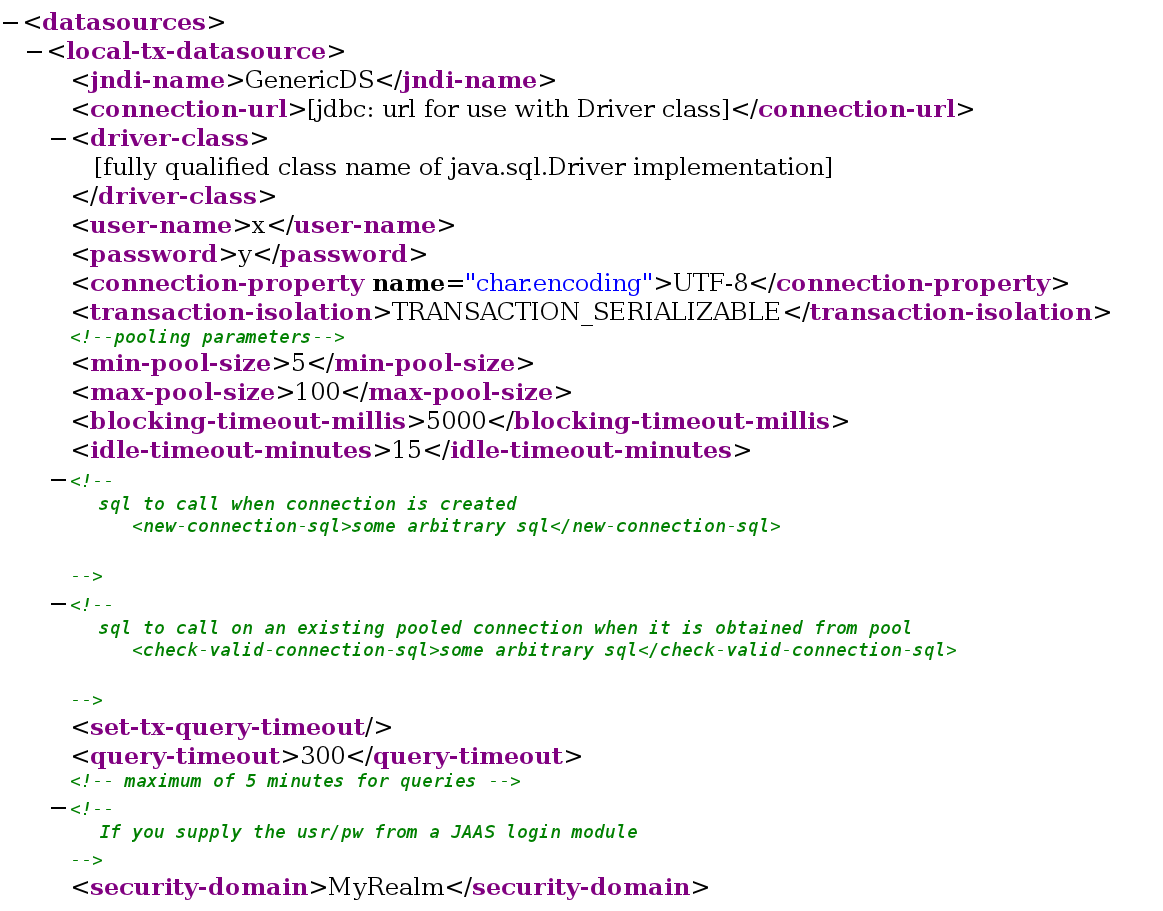
\includegraphics[scale=0.3]{img/datasource.png}
  \end{center}

  \paragraph{} Ce fichier contient donc les informations usuelles de connexion à une base de données
  (nom d'utilisateur, mot de passe, URL de connexion,...) mais aussi un ensemble de paramètre
  spécifique à la ressource utilisée (nom du \textit{driver} Java à utiliser, durée maximum d'attente
  d'une connexion - \textit{timeout}, de type de support transactionnel, etc...). On peut donc ainsi
  facilement modifier le base de données utilisée, ainsi que son comportement, selon que l'on soit,
  par exemple, en développement ou en production.
}

\ifslide {
  \begin{frame}{Base de donnée relationnelle (SQL)}
    \begin{center}
      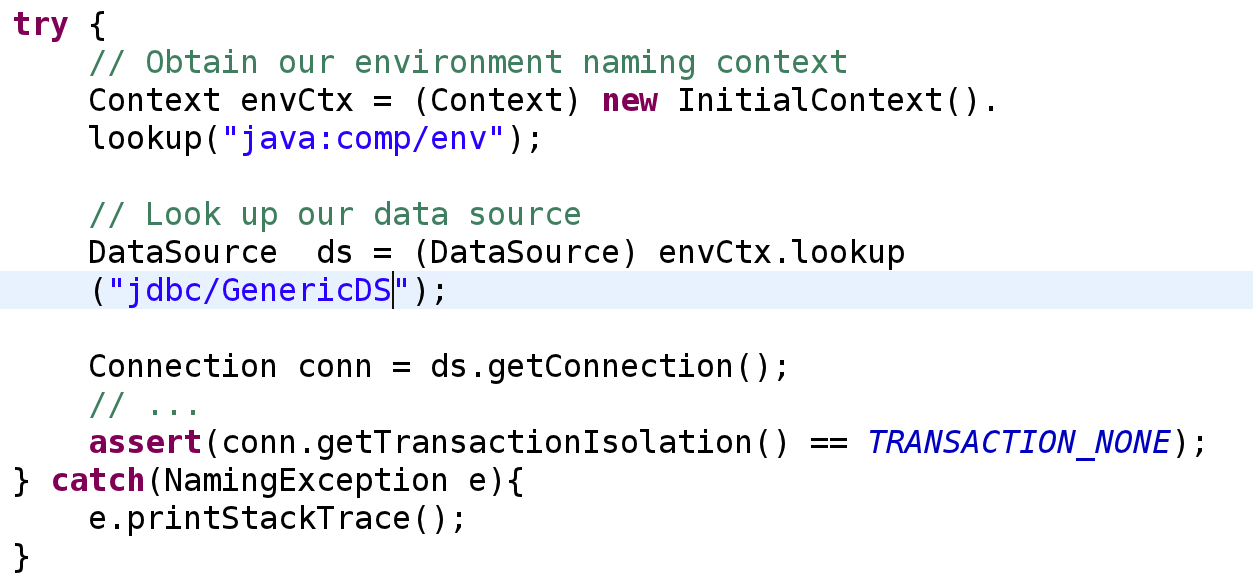
\includegraphics[scale=0.3]{img/datasource-connection.png}
    \end{center}
  \end{frame}

  \begin{frame}{Base de donnée relationnelle (SQL)}
    \begin{center}
      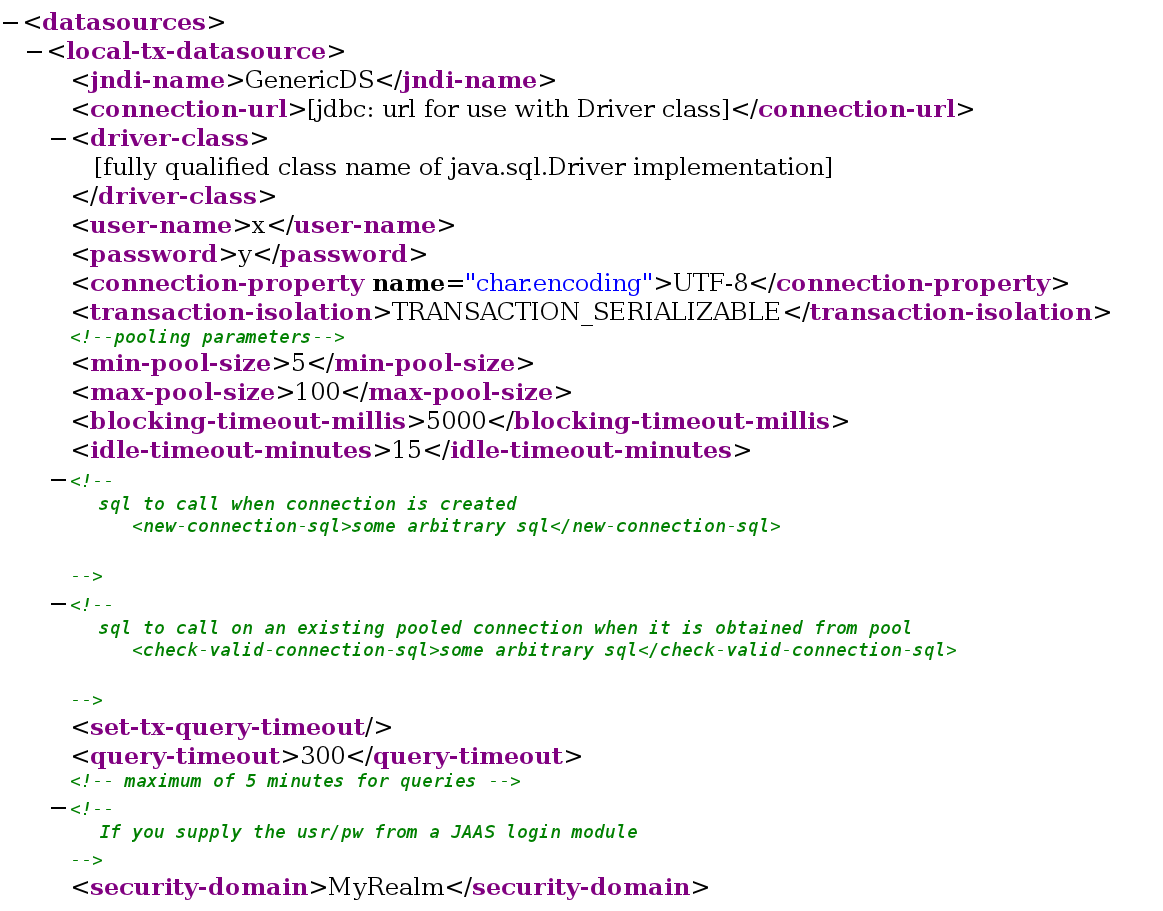
\includegraphics[scale=0.3]{img/datasource.png}
    \end{center}
  \end{frame}

  \begin{frame}{Pilote de base de données}
    \begin{center}
      
\includegraphics[scale=0.05]{../img/pilot.jpg}
      \myphotocredit{http://www.flickr.com/photos/maticevic/4595046244/sizes/o/in/photostream/}{Andrea Maticevic}
    \end{center}
    \begin{block}{Pourquoi utiliser un pilote pour une base de données ?}
      \begin{itemize}
        \item offre une API pour communiquer avec la base de données
        \item fournit le gestionnaire de connexion
        \item support (+/-) paramétrable pour les transactions
        \item optimisation côté client
      \end{itemize}
    \end{block}
  \end{frame}
}

\ifbook {
  \mysubsubsection{Annuaire}

  \paragraph{} Le second exemple que nous allons étudier est probablement presque aussi courant que
  l'utilisation de base de données relationnelle. Il s'agit de l'utilisation, par une application,
  d'un annuaire, dont le schéma et le protocole suivent, la plupart du temps, le standard
  \mylink{TODO}{LDAP}. Comme nous allons sommairement le voir, cette nouvelle ressource, pourtant de
  nature très différente, se présente de la même manière à l'application.

  \paragraph{} En effet, l'extrait de code ci dessous, qui présente le code Java standard à utiliser
  pour se connecter à un \textit{pool} de connexion vers un annuaire LDAP, ressemble pour beaucoup à
  celui présenté dans la précédente section:

  \begin{center}
    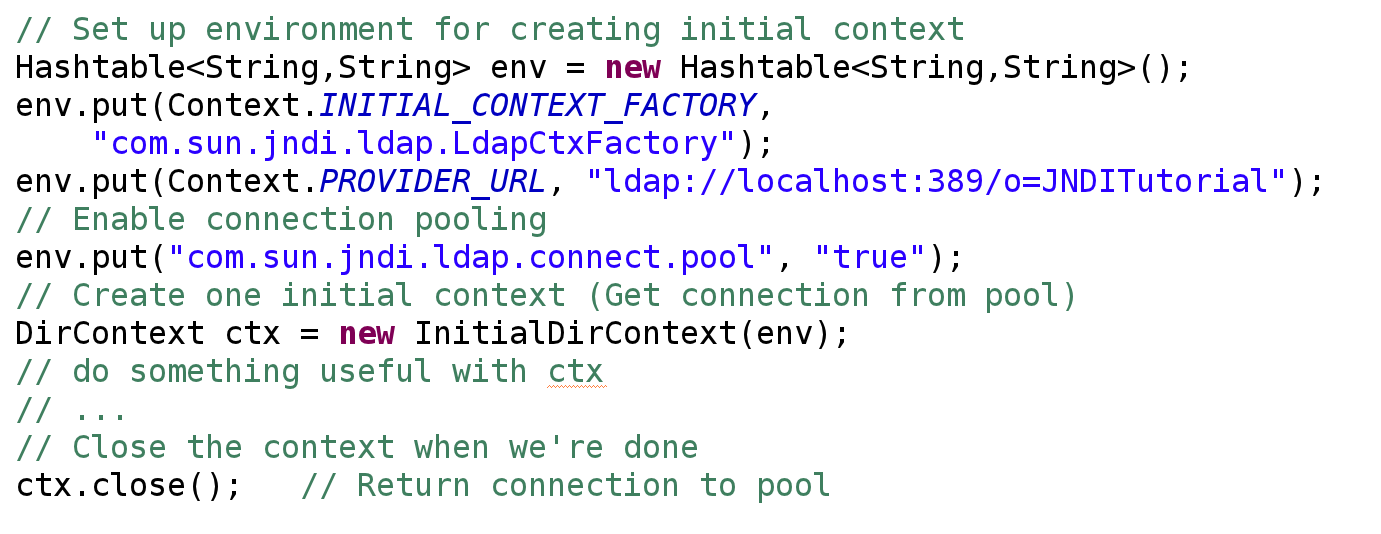
\includegraphics[scale=0.3]{img/ldap-pooling.png}
  \end{center}
}

\ifslide{
  \begin{frame}{Qu'est ce qu'un annuaire LDAP ?}
    \begin{block}{Fonctions d'un LDAP}
      \begin{itemize}
        \item base de données \textbf{hiérarchique}
        \item conçu pour stocker un \textbf{annuaire d'entreprise}
        \item protocole dédié et \textbf{standard}
        \item persistance d'une structure hiérarchique
      \end{itemize}
    \end{block}

    \begin{center}
      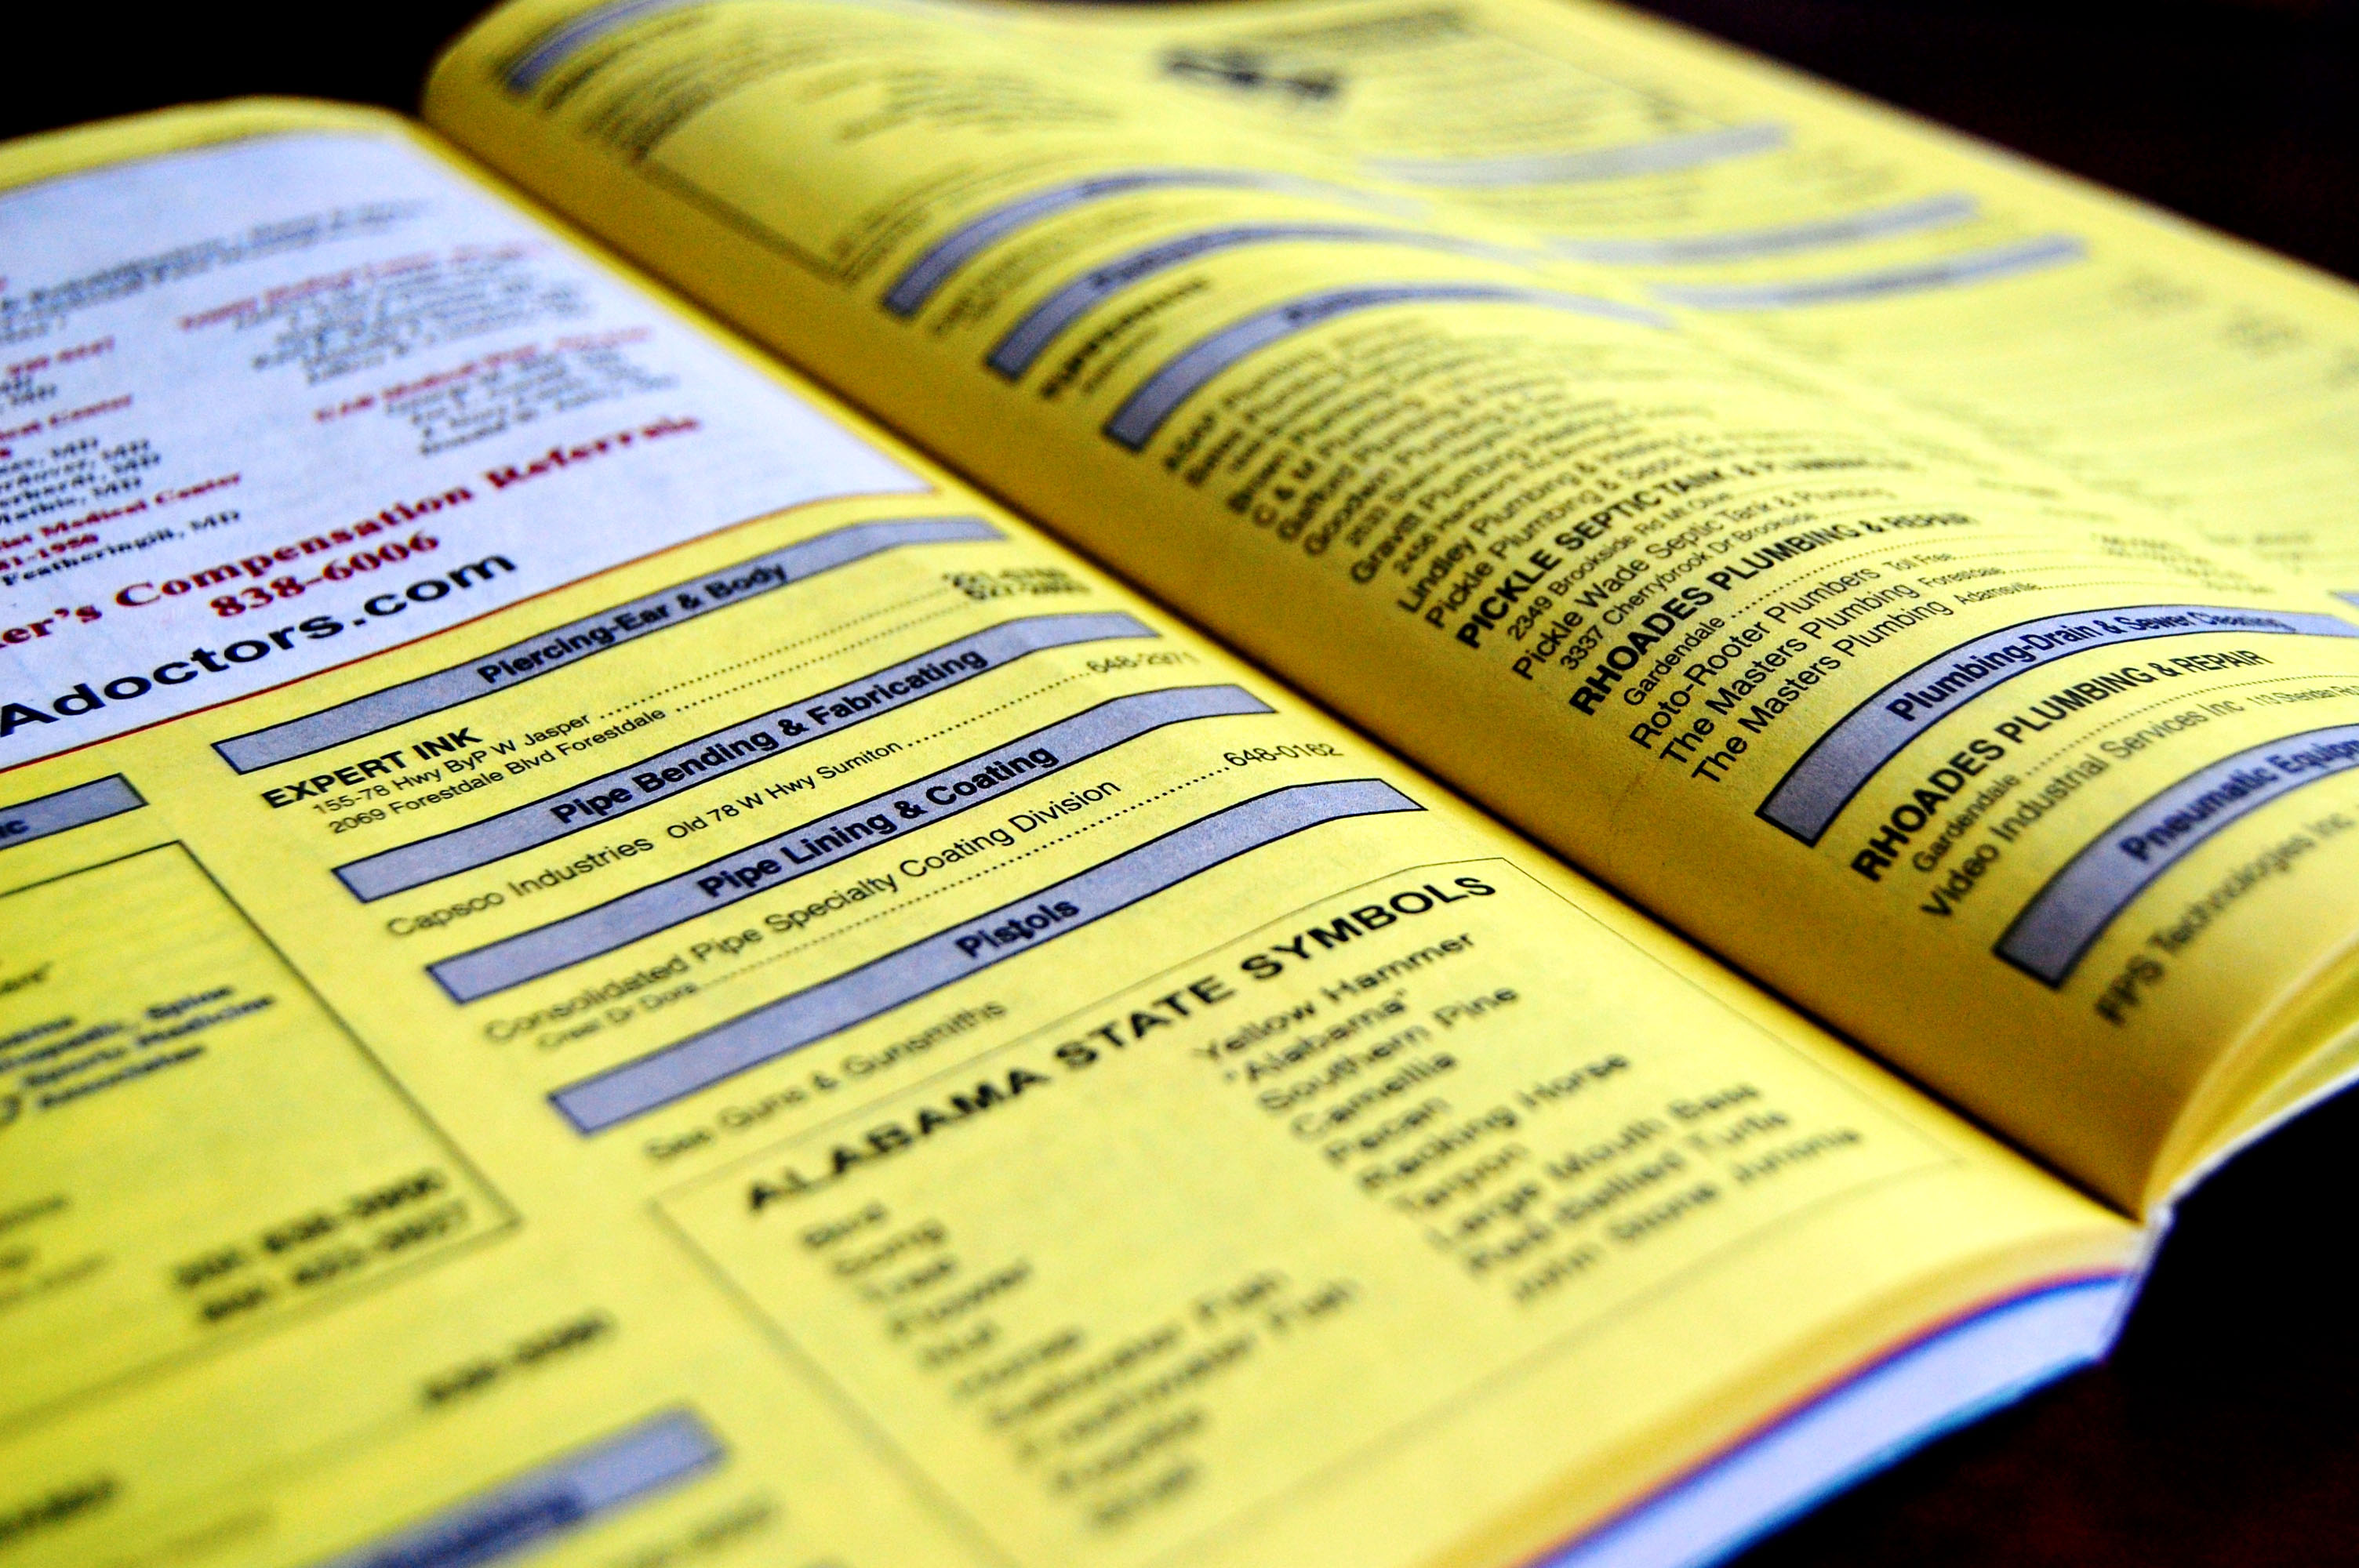
\includegraphics[scale=0.2]{../img/yellow-pages.jpg}
      \myphotocredit{http://www.flickr.com/photos/jamiesrabbits/4248396588/lightbox/}{Jamiesrabbits}
    \end{center}
  \end{frame}
}

\ifbook{
  \mysubsubsection{NoSQL}

  \paragraph{} Si les bases de données et les annuaires font parti du paysage des systèmes
  d'informations depuis maintenant fort longtemps, il apparait important de prolonger cette partie
  pour évoquer ces nouvelles ressource que sont les bases de données \textit{NoSQL}.

  \paragraph{} Commençons d'ailleurs par souligner que ces dernières ne construisent pas forcément en
  opposition au modèle SQL - comme leur nom pourrait sous entendre, mais comme une alternative ou
  plus souvent comme complémentaire à l'usage de base de données SQL. En effait, l'acronyme
  \textit{NoSQL} signifie en \textit{"Not Only SQL"\footnote{Traduction: Pas seulement du SQL}}.

  \paragraph{} Ces ressources utilisent d'autres mécanismes, que ceux promût par les bases de données
  relationnelles, pour effectuer la persistance et/ou la recherche de données. Parmi les stratégies
  les plus courantes, nous pouvons nommer les suivants:

  \begin{itemize}
    \item clé/valeur (\mylink{TODO}{Memcached})
    \item document (\mylink{TODO}{Mongodb})
    \item graphe (\mylink{TODO}{Neo4j})
    \item objet (\mylink{TODO}{db4o})
    \item "hybride" (\mylink{TODO}{infinite span})
  \end{itemize}

  \paragraph{} Présenter en détail ces différents mécanismes dépasse largement le contexte de ce
  cours. Ce qu'il est important de retenir dans le contexte du \textit{middleware} est que ces
  nouvelles bases de données demeurent des \textbf{ressource} et que donc l'ensemble des
  problématiques évoqués dans cette section (gestionnaire de connexion, authentification, sécurité,
  transaction,...) s'appliquent tout autant à elles qu'à leurs prédécesseurs.

  \paragraph{} Si leur utilisation, dans le cadre de la réalisation d'une application peut très
  certainement se révéler judicieuse et apporter une approche plus adaptée à la problématique
  adressée, elles ne sont en aucun des solutions miracles, et les difficultés rencontrées avec les
  ressources plus traditionnelles, feront tout autant surface avec elles.
}

\ifslide{
  \begin{frame}{NoSQL}
    \begin{block}{Base NoSQL}
      \begin{itemize}
        \item reste des ressource
        \item plus ou moins configurable
        \item moins standard
        \item plus "sexy"
      \end{itemize}
    \end{block}

    \begin{block}{Fonctionnement}
      \begin{itemize}
        \item clé/valeur (memcached)
        \item document (mongodb)
        \item graphe (neo4j)
        \item objet (db4o)
        \item "hybride" (infinite span)
      \end{itemize}
    \end{block}

  \end{frame}

  \begin{frame}{InfiniSpan}
    \begin{center}
      
\includegraphics[scale=0.2]{../img/infinispan-logo.png}
    \end{center}

    \begin{block}{Un exemple de base de données NoSQL}
      \begin{itemize}
        \item grille de données
        \item montée en charge linéaire
        \item pas de contrainte de relation
        \item parfait pour des opérations de lecture
      \end{itemize}
    \end{block}
  \end{frame}

  \begin{frame}{InfiniSpan - Cas pratique}
    \begin{center}
      Mise en place d'un SSO inter site
      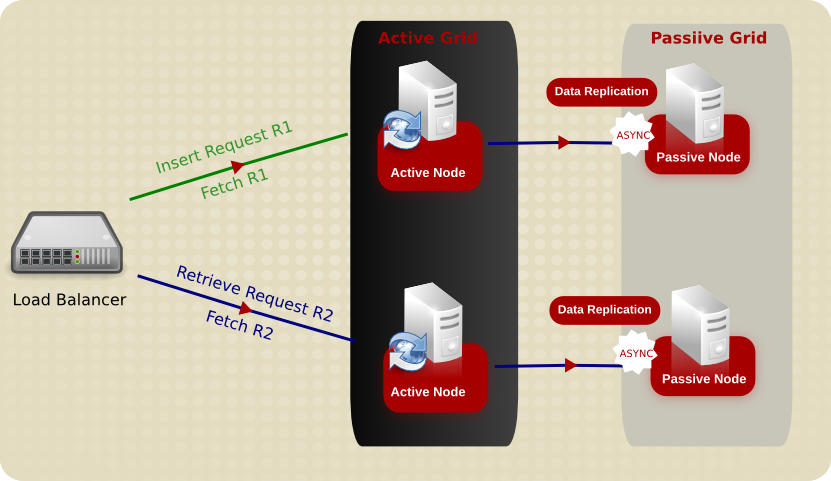
\includegraphics[scale=0.4]{../img/infinispan-example.png}
    \end{center}
  \end{frame}

  \begin{frame}{Base de données spécialisées}
    \begin{block}{Qu'est ce qu'une base de données spécialisés ?}
      \begin{itemize}
        \item orienté ou optimisé pour un certain modèle de données
        \item produit indépendant ou construit sur une base de données "généraliste"
        \begin{itemize}
         \item PostGIS - extension géospatial pour Postgresql
        \end{itemize}
      \end{itemize}
    \end{block}
    \begin{center}
      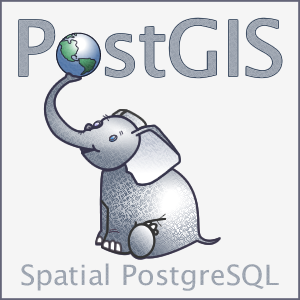
\includegraphics[scale=0.4]{../img/PostGIS-database.png}
    \end{center}
  \end{frame}

  \begin{frame}{ETL, un exemple d'outil}
    \begin{center}
      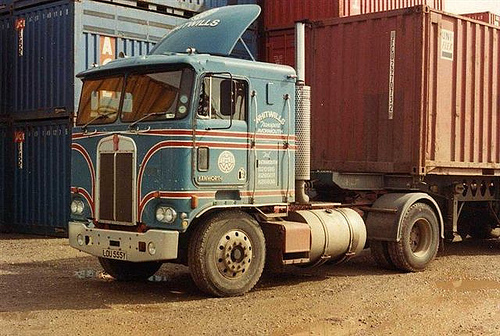
\includegraphics[scale=0.4]{../img/truck.jpg}
    \end{center}

    \begin{block}{Propos et intérêt des ETLs}
      \begin{itemize}
        \item \textit{Extract, Transform, Load}
        \item migrer les données d'une base de données à une autre
        \begin{itemize}
          \item importer depuis Oracle une base de données dans Postgresql
          \item intégrer dans un entrepôt de données (\textit{datawharehouse})
        \end{itemize}
      \end{itemize}
    \end{block}
  \end{frame}

  \begin{frame}{ETL, un exemple d'outil}
    \begin{center}
      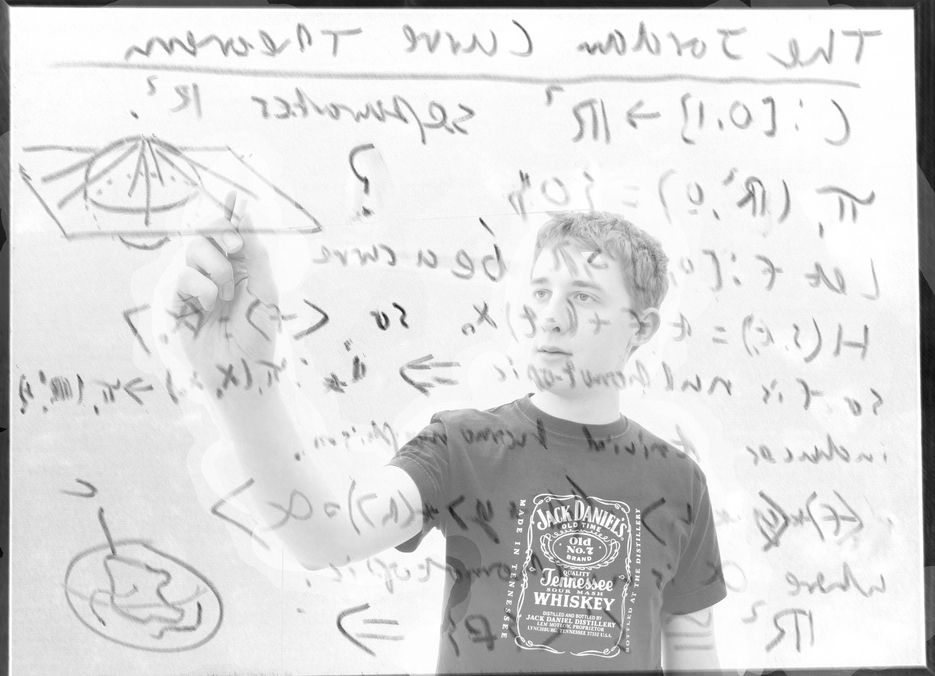
\includegraphics[scale=0.1]{../img/math.jpg}
    \end{center}
    \begin{block}{Transformation de données}
      \begin{itemize}
        \item conversion de données (ex:"1" à "M", "0" en "F")
        \item calcul dérivé (ex: gain = quantité * prix)
        \item ajout de clé étrangère
        \item jointure de données de source différente
      \end{itemize}
    \end{block}
  \end{frame}
}
